\documentclass[a4paper]{article}

\usepackage[romanian]{babel}
\usepackage{amsmath}
\usepackage{indentfirst} % indenteaza primul paragraf din fiecare sectiune
\usepackage{graphicx}
\usepackage{hyperref}
\usepackage{caption}
\usepackage{subcaption} % pentru subfiguri
\usepackage{enumitem}

\renewcommand{\phi}{\varphi} % use phi from amsmath
\renewcommand{\Omega}{\varOmega} % use Omega from amsmath

\title{Referat: Studiul miscarii oscilatorii
cu ajutorul pendulului de torsiune}
\author{Nicolas Dumitru}

\begin{document}

\maketitle

\section{Scopul lucrării}
\begin{enumerate}
	\item{Analiza oscilatiilor libere}
	      \begin{enumerate}
		      \item determinarea momentului
		            de torsiune prin metoda
		            statică şi prin metoda
		            dinamică
		      \item determinarea frecvenţei
		            proprii a oscilatorului
		            liber amortizat şi a
		            perioadei proprii de
		            oscilaţie, pentru
		            diferite valori ale
		            amortizării şi
		            determinarea momentului
		            de inerţie al pendulului
		      \item determinarea
		            coeficientului de
		            amortizare, a timpului
		            de relaxare şi a
		            decrementului logaritmic

	      \end{enumerate}
	\item{Analiza oscilatiilor fortate}
	      \begin{enumerate}
		      \item trasarea curbei de rezonanta a
		            oscilatorului forţat pentru diferite amortizări;
		      \item determinarea frecvenţei de rezonanţă;
		      \item analiza diferenţei de fază dintre
		            oscilator şi forţa exterioară pentru diferite
		            frecvenţe de forţare (foarte mici sau foarte
		            mari comparativ cu frecvenţa de rezonanţă).
		      \item determinarea factorului de calitate al
		            oscilatorului pentru diferite amortizări
	      \end{enumerate}
\end{enumerate}

\section{Teoria lucrării}
Mișcarea unui pendul de torsiune este descrisă de ecuația diferențială
\begin{equation}
	I \frac{d^2 \phi}{dt^2} + k_{fr} \frac{d \phi}{dt} + C \phi = 0
\end{equation}

unde $I$ --- momentul de inerție; $\phi$ --- unghiul de rotație; $k_{fr}$ ---
constanta de frecare; $C$ --- constanta de torsiune.

Folosind relațiile uzuale: $\omega_0^2 = \frac{C}{I}$ --- pulsația proprie $\delta =
	\frac{k_{fr}}{2I}$ --- coeficient de amortizare, ecuația devine:

\begin{equation}
	\frac{d^2 \phi}{dt^2} + 2 \delta \frac{d \phi}{dt} + \omega_0^2 \phi = 0 \text{.}
\end{equation}

În rezolvarea acestei ecuații diferențiale liniare de ordinul 2 intervin 3
situații distincte:

\begin{itemize}
	\item Cazul A: $\omega_0^2 > \delta^2$ (regim sub-amortizat) \\
	      Soluția: \\
	      \begin{equation}
		      \phi = \phi_0 e^{-\delta t} \cos \omega t
	      \end{equation}
	      cu $\phi_0$ --- amplitudinea unghiulara la momentul
	      inițial și $\omega = \sqrt{\omega_0^2 - \delta^2}$
	      --- pulsația oscilațiilor amortizate indică o
	      descreștere a amplitudinii. \textbf{Timpul de relaxare}:
	      \begin{equation}
		      \frac{\phi(t)}{\phi(t + \tau)} = \frac{1}{e} \implies \tau = \frac{1}{\delta}
	      \end{equation}
	      Logaritmul raportului valorilor amplitudinilor după
	      o perioadă se numește \textbf{decrement logaritmic}
	      și se definește conform relației:
	      \begin{equation}
		      D = \ln \frac{\phi(t)}{\phi(t + T)} = \delta T \text{.}
	      \end{equation}
	\item Cazul B: $\omega_0^2 < \delta^2$ (regim supra-amortizat). \\
	      Soluția este aperiodică, de forma:
	      \begin{equation}
		      \phi = \phi_0 e^{-\delta t}(e^{\omega t} + e^{-\omega t})
	      \end{equation}
	      Sistemul revine asimptotic spre poziţia de echilibru
	      după o singură oscilaţie.
	\item Cazul C: $\omega_0^2 = \delta^2$ (regim supra-amortizat critic).
	      Soluția este:
	      \begin{equation}
		      \phi = (\phi_0 + Bt) e^{-\delta t}
	      \end{equation}
	      Sistemul revine în poziţia iniţială de unde nu mai
	      pleacă. Acest caz are importanţă
	      practică deoarece sistemul ajunge în timpul cel mai
	      scurt în poziţia de echilibru.
\end{itemize}

Pentru ca mişcarea să nu se amortizeze în timp, fenomenele de frecare
responsabile de disiparea energiei trebuie compensate din exterior, prin
furnizarea unei energii suplimentare. Acest lucru se poate realiza prin
aplicarea unei forţe periodice ce produce un moment de torsiune periodic asupra
pendulului:
\begin{equation}
	M = M_0 \cos \Omega t \text{.}
\end{equation}
Ecuația de mișcare devine:
\begin{equation}
	\frac{d^2 \phi}{dt^2} + 2 \delta \frac{d \phi}{dt} + \omega_0^2 \phi = f
	\cos \Omega t
\end{equation}
unde $f_0 = \frac{M_0}{I}$.

După regimul tranzitoriu, se instalează regimul staționar, cu soluția de forma:
\begin{equation}
	\phi(t) = A \cos(\Omega t - \phi) \text{.}
\end{equation}

Amplitudinea A:
\begin{equation}
	A = \frac{f_0}{\sqrt{(\omega_0^2 - \Omega^2)^2 + (2 \delta \Omega)^2}}
\end{equation}
\begin{equation}
	A = \frac{f_0 / \omega_0^2}{\sqrt{\left(1 -
			\left(\frac{\Omega}{\omega_0}\right)^2\right)^2 + \left(2
			\frac{\delta}{\omega_0} \frac{\Omega}{\omega_0} \right)^2}}
\end{equation}

Concluzii:
\begin{itemize}
	\item $A$ creşte direct proporţional cu valoarea forţării exterioare, $f_0$
	\item $A$ atinge o valoare maximă (fenomen numit rezonanţa amplitudinii) pentru o anumită valoare a
	      frecvenţei forţării, care se determină din relaţia
	      $dA / d\Omega = 0$. Frecvența de rezonanță:
	      $\Omega_r = \sqrt{\omega_0^2 - 2 \delta^2}$
	\item $A$ scade odată cu creșterea $\delta$
	\item Pentru amortizare nulă ($\delta = 0$), $A \to \infty$ dacă $\Omega_r = \omega_0$.
\end{itemize}

\begin{equation}
	\tan \phi_0 = \frac{2 \delta \omega_0}{\omega_0^2 - \Omega^2}
\end{equation}

Pentru $\omega_0 \gg \Omega \implies \phi_0 \to 0$, pendulul oscilează aproape
în fază cu sursa.

Pentru $\omega_0 \ll \Omega \implies \phi_0 \to \pi$, pendulul
oscilează aproape în antifază cu sursa.

Pentru $\omega_0 = \Omega \implies \phi_0 \to \pi / 2$.

\section{Schițe și grafice}
\begin{figure}[htbp]
	\centering
	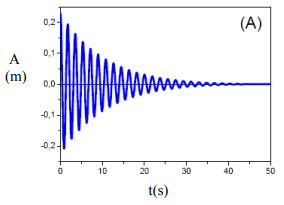
\includegraphics[width=0.3\textwidth]{subamortizata.png}
	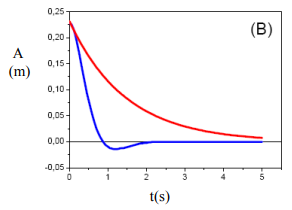
\includegraphics[width=0.3\textwidth]{supraamortizata.png}
	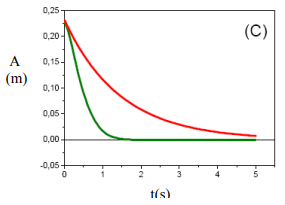
\includegraphics[width=0.3\textwidth]{amortizata_critic.png}
	\caption{Reprezentarea grafică a
		amplitudinii (A) pentru tipuri
		diferite de mişcări amortizate: (A)
		subamortizată; (B) supraamortizată;
		(C) amortizată critic}
	\label{fig:grafice_amortizare}
\end{figure}

\begin{figure}[htbp]
	\centering
	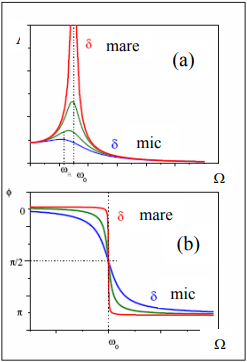
\includegraphics[width=0.3\textwidth]{frecventa_amplitudine_faza.png}
	\caption{Dependenţa de
		frecvenţa forţei exterioare a
		(a) amplitudinii; (b) a
		diferenţei de fază}
	\label{fig:freampfaz}
\end{figure}

\begin{figure}[htbp]
	\centering
	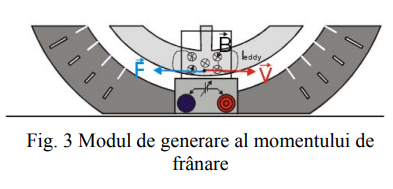
\includegraphics[width=0.3\textwidth]{franare.png}
	\caption{Modul de generare al momentului de
		frânare}
	\label{fig:franare}
\end{figure}

\begin{figure}[hbtp]
	\centering
	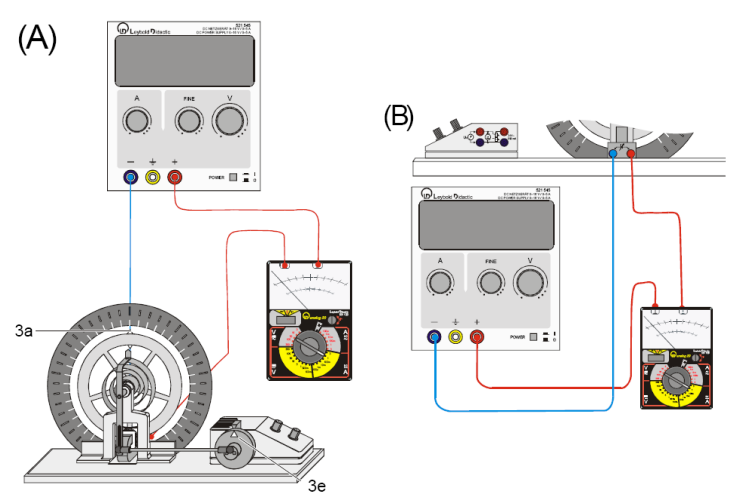
\includegraphics[width=0.5\textwidth]{device.png}
	\caption{Montajul experimental (A) cu detalii asupra conexiunilor electrice
		(B)}
	\label{fig:device}
\end{figure}

\end{document}
